\documentclass[aspectratio=169]{beamer}
\usepackage{amssymb,amsmath}
\usepackage{graphicx}
\usepackage{url}
\usepackage{color}
\usepackage{pagenote}[continuous,page]
\usepackage{cancel}   % Math "cancelto"
\usepackage{relsize}	% For \smaller
\usepackage{url}			% For \url
\usepackage{epstopdf}	% Included EPS files automatically converted to PDF to include with pdflatex

%For MindMaps
\usepackage{tikz}%
\usetikzlibrary{mindmap,trees,arrows}%

%%% Color Definitions %%%%%%%%%%%%%%%%%%%%%%%%%%%%%%%%%%%%%%%%%%%%%%%%%%%%%%%%%
%\definecolor{bordercol}{RGB}{40,40,40}
%\definecolor{headercol1}{RGB}{186,215,230}
%\definecolor{headercol2}{RGB}{80,80,80}
%\definecolor{headerfontcol}{RGB}{0,0,0}
%\definecolor{boxcolor}{RGB}{186,215,230}

%%% Save space in lists. Use this after the opening of the list %%%%%%%%%%%%%%%%
%\newcommand{\compresslist}{
%	\setlength{\itemsep}{1pt}
%	\setlength{\parskip}{0pt}
%	\setlength{\parsep}{0pt}
%}

%\setbeameroption{show notes on top}

% You should run 'pdflatex' TWICE, because of TOC issues.

% Rename this file.  A common temptation for first-time slide makers
% is to name it something like ``my_talk.tex'' or
% ``john_doe_talk.tex'' or even ``discrete_math_seminar_talk.tex''.
% You really won't like any of these titles the second time you give a
% talk.  Try naming your tex file something more descriptive, like
% ``riemann_hypothesis_short_proof_talk.tex''.  Even better (in case
% you recycle 99% of a talk, but still want to change a little, and
% retain copies of each), how about
% ``riemann_hypothesis_short_proof_MIT-Colloquium.2000-01-01.tex''?

\mode<presentation>
{
  \usetheme{CambridgeUS}
  \usecolortheme{dolphin}
  \useoutertheme{default}
  \useinnertheme{default}
  \setbeamercovered{invisible} % or whatever (possibly just delete it)
}
\beamertemplatenavigationsymbolsempty

\usepackage[english]{babel}
%\usepackage[latin1]{inputenc}
\usepackage{subfigure}

\usepackage{times}
\usepackage[T1]{fontenc}
\usepackage{CJKutf8}

%% makes the ppagenote command for figure references at the end.
\makepagenote
\renewcommand{\notenumintext}[1]{}
\newcommand{\ppagenote}[1]{\pagenote[Page \insertframenumber]{#1}}

\title[Experiment Design (01CH740)]{Experiment Design for Computer Sciences (01CH740)}
\author[Claus Aranha]{Claus Aranha\\{\footnotesize caranha@cs.tsukuba.ac.jp}}
\institute[U. Tsukuba]{University of Tsukuba, Department of Computer Sciences}


\subtitle[Experimental Factors]{Topic 07 - Experimental Factors}
\date{}

\begin{document}
\begin{CJK}{UTF8}{ipxm}

\begin{frame}
  \maketitle

  \vfill

  \hfill \tiny{Version 2022.1 (Updated \today)}
\end{frame}

\begin{frame}{Outline}
  In this material, we study simple strategies for handling experiments with {\bf multiple factors}.
  \bigskip

  \begin{itemize}
    \item One Variable at a Time Design (OVAT)
    \item Blocking Design
    \item Factorial Design
  \end{itemize}
\end{frame}

\section{One Variable at a Time}
\begin{frame}
  \begin{center}
    {\bf Part I -- One Variable At a Time (OVAT)}
  \end{center}
\end{frame}

\begin{frame}{Factors and Levels}
  \begin{itemize}
    \item {\bf Factors}: Input variables in the experiment / "control variables";
    \item {\bf Levels}: The values that a factor can assume / "treatments";
  \end{itemize}

  \begin{block}{Example: Carrying Speed Experiment}
    I want to measure how the weight of my luggage affects my speed. I measure
    how far I walk in 5 minutes, when carrying 10, 20 and 40kgs of luggage.\bigskip

    \begin{itemize}
      \item Response Variable: distance walked in 5 minutes;
      \item Factors: Weight of luggage;
      \item Levels: 10kgs, 20kgs, 40kgs;
    \end{itemize}
  \end{block}
\end{frame}


\begin{frame}{Experiments with One Factor}
  Until now, we considered experiments with 1 factor and 1 return variable;
  \begin{itemize}
    \item {\bf t-test}: 1 factor, two levels
    \item {\bf ANOVA}: 1 factor, many levels
  \end{itemize}

  \begin{block}{Example}
    We want to compare how long it takes to train a neural network until a certain
    error value is reached. We compare four optimization algorithms: SGD, Adam, Adagrad, CMA-ES.

    \begin{itemize}
      \item Response Variable: Time until error threshold is reached;
      \item Factor: Optimization Algorithm;
      \item Levels: 1- SGD, 2- Adam, 3- Adagrad, 4- CMA-ES
    \end{itemize}
  \end{block}
\end{frame}

\begin{frame}{Experiment with Two Factors}
  \begin{block}{
    We add a new factor to the experiment: The number of layers
    in the network (2, 5 or 10)}
    \begin{itemize}
      \item Response Variable: Time until error threshold is reached;
      \item Factor 1, 4 levels: Optimization Algorithm: SGD, Adam, Adagrad, CMA-ES;
      \item Factor 2, 3 levels: 2, 5, 10 layers;
    \end{itemize}
  \end{block}

  \begin{itemize}
    \item {\bf Experiment with 1 factor:} Only consider the effect of the levels on the response variable.
    \item {\bf Experiment with 2 factors:} Consider main effect and interference effects:
    \begin{itemize}
      \item {\bf Main Effect:} Effect of the levels of each factor in the response variable.
      \item {\bf Interaction Effects:} Combined effects of levels of both factors in the response variable.
    \end{itemize}
  \end{itemize}

\end{frame}

\begin{frame}{Number of Factors and Experiment Complexity}

  The higher the number of factors and levels, the more complex becomes the experiment.
  \begin{itemize}
    \item 2 factors, 4 levels each: 16 total combinations; 2nd order interactions;
    \item 3 factors, 3 levels each: 27 total combinations; 3rd order interactions;
    \item 4 factors, 3 levels each: 81 total combinations; 4th order interactions;
    \item ...
  \end{itemize}\bigskip

  Because of this, it is desirable to keep experiments simple, even if there are statistical techniques to detect interaction effects.
\end{frame}

\begin{frame}{OVAT -- One Variable at a Time}
  The simplest design to use with multiple factors is the OVAT Design.\bigskip

  \begin{itemize}
    \item For $N$ factors, perform $N$ different experiments, one for each factor.
    \item The levels of the other factors are fixed at a "standard" value.
    \item For each factor, you perform the statistical analysis independently (t-test, anova, visualizations, etc);
  \end{itemize}
\end{frame}

\begin{frame}{OVAT -- Example}
  \begin{block}{Fine tuning Cr and F for Differential Evolution (DE)}
    DE is an effective optimization algorithm where the performance depends
    strongly on two parameters: Cr and F.\bigskip

    To find the optimal values for these parameters, you perform a preliminary
    experiment on a synthetic benchmark.
  \end{block}

  OVAT Design:
  \begin{itemize}
    \item Choose standard values for Cr and F from the literature.
    \item Analyze Cr using an experiment. Fix the value of F and try 10
      different values (levels) for CR.
    \item Analyze F using another experiment. Fix the value of Cr and try 10
      different values (levels) for F.
    \item The execution and analysis of these two experiments follow the
      methods that we already studied.
  \end{itemize}
\end{frame}




























%

\section{Blocking Design}
\begin{frame}
  \begin{center}
    {\bf Part II - Blocking Design}
  \end{center}
\end{frame}

\begin{frame}{Completely Randomized Design (CRD)}
  Until now, we studied the following situation:
  \begin{itemize}
    \item One input factor (for example, algorithm type)
    \item One response variable (for example, solution speed)
    \item An {\bf homogeneous experimental condition}.
  \end{itemize}\bigskip

  \begin{block}{Homogeneous experimental condition}
    This means that the experiment environment is guaranteed to be the same
    for all observations, and there are no significant error sources.
  \end{block}\bigskip

  In this situation, we execute the experiment in {\bf random order} to
  guarantee that any error sources are equally distributed.
  We call this a {\bf Completely Randomized Design (CRD)}
\end{frame}

\begin{frame}{Block Design}

  {\bf Noise / Nuisance Factors} are input variables that can have a significant impact in
  the experiment output, but they are not relevant to the scientific question.\bigskip

  In a previous lecture, we discussed the use of {\bf Pairing} to remove the
  effect of \emph{one} noise factor. {\bf Blocking} is the generalization of the
  Paired Design approach for multiple noise factors.\bigskip

  \begin{block}{Block Design vs Completely Randomized Design}
    We use Randomization (CRD) to prevent the effect of \emph{unknown} noise factors in our experiment.
    \bigskip

    We use Blocking or Pairing when we know from the beginning that certain factors affect the output
    variable, but for some reason we are not interested in their effects.
  \end{block}
\end{frame}

\subsection{Example Problem}
\begin{frame}{Example of Block Design}{Algorithm Comparison}

  A student decides to compare a standard optimization algorithm against
  size variants to solve a certain family of Vehicle Routing Problems (VRPs).
  \bigskip

  He wants to know if any variant returns a systematically lower cost value,
  when applied to 180 problem instances. These instances can be divided in
  {\bf 36 groups}, with 5 similar instance in each group.


  \begin{columns}
    \column{.8\textwidth}
    \begin{block}{Experiment Design Variables}
      \begin{itemize}
        \item confidence: $\alpha = 0.05$
        \item power: $\pi = 1 - \beta = 0.8$
        \item minimally interesting effect: $\delta^* = 50$
      \end{itemize}
    \end{block}
    \column{.2\textwidth}
    
\includegraphics[width=1\textwidth]{../img/phdStudent.png}
    \ppagenote{PhD Student Image: PhD Comics by Jorge Cham, http://www.phdcomics.com/comics/archive.php?comicid=1139}
  \end{columns}
\end{frame}

\begin{frame}{Example of Block Design: Factors and levels}
  For this problem, we can identify the following variables:
  \begin{itemize}
    \item {\bf Input Factor}: Algorithm; {\bf Levels:} Original and 6 variants;
    \item {\bf Return Variable}: Cost; {\bf Levels:} Integer value;
    \item {\bf Noise Factor}: Instance type; {\bf Levels:} 36 groups;
  \end{itemize}\bigskip

  If we employ a CRD (ignoring or randomizing the Noise Factor), the difference
  in result among Instance types would have an effect in the residual, and possibly mask
  the difference between algorithms.\bigskip

  To avoid this, we organize the experiment in 36 blocks (one block per level of
  the Noise Factor), and randomize the execution of all 7 algorithms inside each block.
  This is the {\bf Randomized Complete Block Design (RCBD)}
\end{frame}

\begin{frame}{Assumptions of the RCBD}
  The RCBD assumes the following characteristics for the experiment:
  \begin{enumerate}
    \item one replicate per block;
    \item the blocks are independent;
    \item randomization inside the block is independent;
  \end{enumerate}\bigskip

  These assumptions are important. If we fail to guarantee the
  independence between the blocks (for example, some of the blocks are dependent),
  we introduce something called {\bf pseudoreplication}, which may result in
  an inflation of type-I error.
\end{frame}

\begin{frame}{Example: Pre-processing the data}
  In the algorithm example, we obtain the following experimental data:
  \begin{itemize}
    \item 7 algorithm variants,
    \item 180 total problem instances, 36 instance group (5 instances per group)
    \item 30 repetitions, per algorithm, per instance (7x30x180 = 37800 observations)
  \end{itemize}\bigskip

  However, as explained in the last slide, the RCBD requires {\bf 1 replicate per block}.
  To satisfy this requirement, we pre-process the data as follows:
  \begin{itemize}
    \item The performance of each algorithm, per instance, is averaged (average of 30 repetitions)
    \item The performance of each algorithm, per group, is averaged (average of 5 instances)
  \end{itemize}
  This gives us 36 observations per algorithm (1 observation per block)
\end{frame}

\begin{frame}[fragile]{Example: Pre-processing the data (R code)}

{\smaller
\begin{verbatim}
> data <- read.table("../data files/algo.csv", header = TRUE)
# Aggregate data (algorithm means by instance group)
> aggdata <- with(data, aggregate(x   = Result, by  = list(Algorithm, Group),
                                  FUN = mean))
# Rename columns and coerce factor variables
> names(aggdata) <- c("Algorithm", "Instance_Group", "Y")
> for (i in 1:2) aggdata[, i] <- as.factor(aggdata[, i])
> levels(aggdata$Algorithm) <- c("Original", unlist(lapply(X   = "Mod",
                                               FUN = paste0, 1:6)))
> summary(aggdata)
    Algorithm  Instance_Group       Y
 Original:36   1      :  7    Min.   : 227.3
 Mod1    :36   2      :  7    1st Qu.: 440.0
 Mod2    :36   3      :  7    Median : 756.8
 Mod3    :36   4      :  7    Mean   : 821.0
 Mod4    :36   5      :  7    3rd Qu.:1020.5
 Mod5    :36   6      :  7    Max.   :2743.6
 Mod6    :36   (Other):210$
\end{verbatim}}
\end{frame}

\begin{frame}[fragile]{Example: Pre-visualization of the Data (R code)}

{\smaller
\begin{verbatim}
> p <- ggplot(aggdata, aes(x = Instance_Group, y = Y,
                           group = Algorithm, colour = Algorithm))
> p + geom_line(linetype=2) + geom_point(size=5)
\end{verbatim}
}

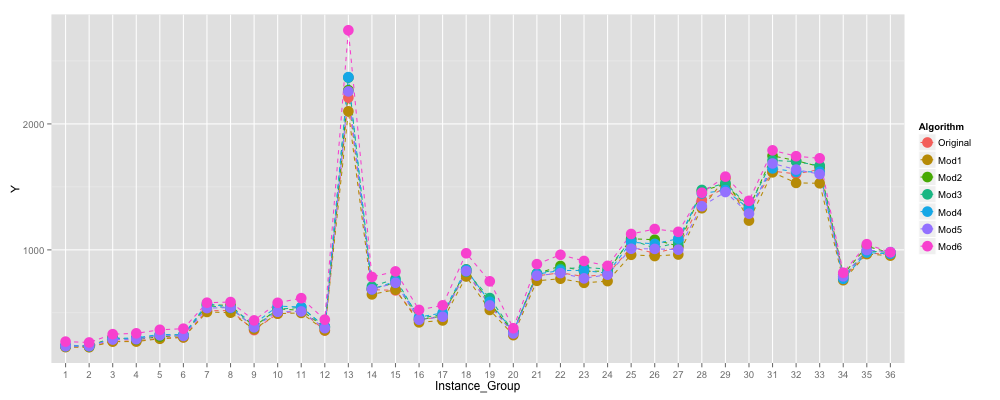
\includegraphics[width=.9\textwidth]{../img/algo_lineplot.png}
\end{frame}

\begin{frame}[fragile]{Statistical Analysis of the CRBD}

The Statistical analysis of the CRBD is similar to the ANOVA analysis we
studied in a previous class. For a derivation of the model, see Campelo in the
recommended readings. \bigskip

However, note that the number of observations is based on the number of blocks
and treatment levels.

{\smaller
\begin{verbatim}
# Anova Model: Treatments+Blocks
> model <- aov(Y~Algorithm+Instance_Group, data=aggdata)

> summary(model)
                Df   Sum Sq Mean Sq F value Pr(>F)
Algorithm        6   359949   59991   41.75 <2e-16 ***
Instance_Group  35 60438639 1726818 1201.86 <2e-16 ***
Residuals      210   301725    1437
---
Signif. codes:  0 '***' 0.001 '**' 0.01 '*' 0.05 '.' 0.1 ' ' 1
\end{verbatim}
}
\end{frame}


\begin{frame}[fragile]{Statistical Analysis of the CRBD -- Residuals}

{\smaller
\begin{verbatim}
> summary.lm(model)$r.squared          # It's important to check the residuals
[1] 0.9950618                          # for anomalies. For example, here
> par(mfrow = c(2, 2))                 # The residual plot shows several outliers
> plot(model, pch = 20, las = 1)       # that could affect the result.
\end{verbatim}}
\centering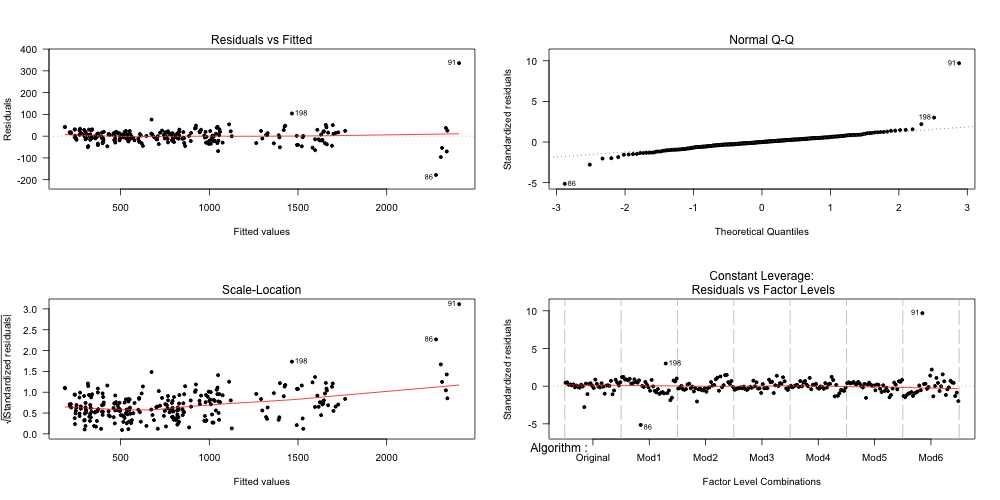
\includegraphics[width=.7\textwidth]{../img/algo_res1.png}
\end{frame}

\begin{frame}[fragile]{Statistical Analysis of the CRBD -- Log Transformation}

An analysis of the residual model showed some irregularities in the
residual plot, so we try a log transformation on the response variable
to see if we can smooth it out.

{\smaller
\begin{verbatim}
# Trying with log-transformed response variable
> model2 <- aov(log(Y)~Algorithm+Instance_Group, data=aggdata)

> summary(model2)
                Df Sum Sq Mean Sq F value Pr(>F)
Algorithm        6   0.60  0.1002   120.4 <2e-16 ***
Instance_Group  35  89.92  2.5690  3089.0 <2e-16 ***
Residuals      210   0.17  0.0008
\end{verbatim}
}
\end{frame}

\begin{frame}[fragile]{Statistical Analysis of the CRBD -- Log Transformation}

{\smaller
\begin{verbatim}
> summary.lm(model2)$r.squared         # The log transformation smoothed out
[1] 0.9980742                          # the outliers from our CRBD model.
> par(mfrow = c(2, 2))                 #
> plot(model2, pch = 20, las = 1)      #
\end{verbatim}}
\centering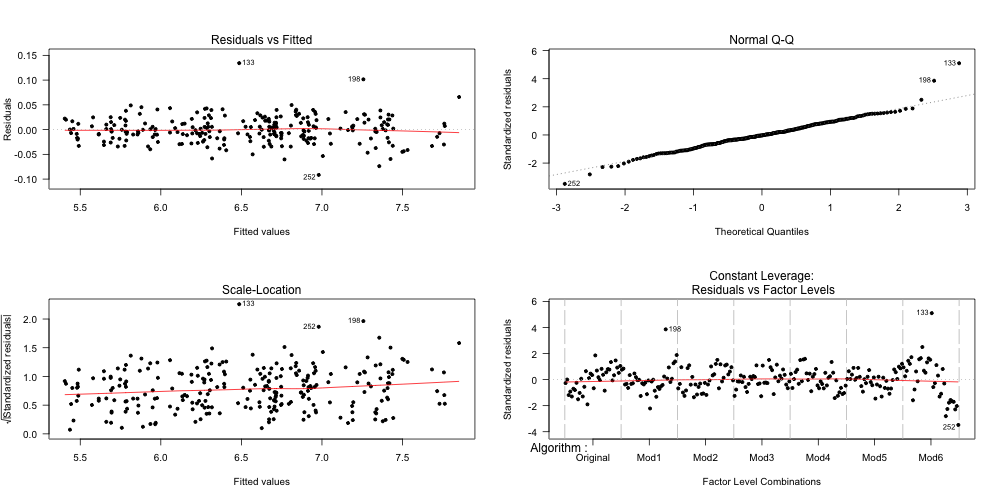
\includegraphics[width=.7\textwidth]{../img/algo_res2.png}
\end{frame}

\begin{frame}{Statistical Analysis of the CRBD -- final comments}
  The post-hoc analysis of the CRBD follows the same principles of the
  post-hoc analysis of the ANOVA.\bigskip

  \begin{itemize}
    \item The type and number of comparisons should be defined a priori.
    \begin{itemize}
      \item In this example, two-sample comparisons between the original algorithm and each variant would be appropriate.
    \end{itemize}
    \item The number of observations should be based on the number of blocks.
    \item Alpha-correction for the paired observations should be applied as necessary.
  \end{itemize}
\end{frame}

\subsection{}
\begin{frame}{Further Reading}
  You should do further reading for these two models that are closely related to the CRBD:
  \begin{itemize}
    \item "Incomplete Block Design" -- When some of the observations (blocks) are missing;
    \item "Generalized Block Design" -- When each block has multiple replicates;
  \end{itemize}
\end{frame}

\section{Factorial Design}
\begin{frame}
  \begin{center}
    {\bf Part III - Factorial Design}
  \end{center}
\end{frame}

\begin{frame}{Factorial Designs}
  Many experiments involve more than one factor of interest. Sometimes we want
  to control {\bf multiple independent variables} that influence the response of the experiment.
  \bigskip

  One effective way to explore the main effects and interactions of multiple factors is
  the {\bf Factorial Design}. In a factorial design, all level combinations are
  explored.\vfill

  \begin{block}{Main Effect and Interaction}
    \begin{itemize}
      \item {\bf Main Effect} of a factor: The mean change of the response variable when we change the level of a factor;
      \bigskip

      \item {\bf Interaction} between factors: The mean change of the response variable when we change the level of two or more factors at the same time.
    \end{itemize}
  \end{block}
\end{frame}

\begin{frame}{Factorial Design Example}

  \begin{columns}
    \column{.1\textwidth}
    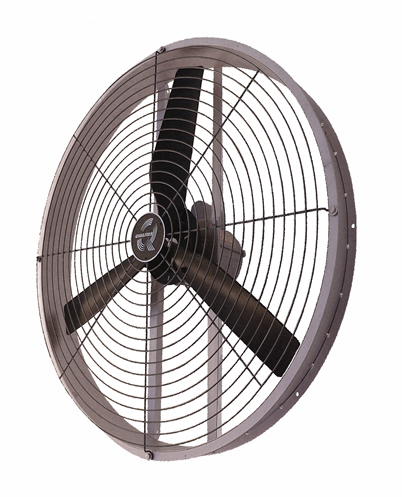
\includegraphics[width=1\textwidth]{../img/ventilador.png}
    \ppagenote{Ventilator figure from http://refrigelms.com.br}
    \column{.9\textwidth}
    An engineer wants to investigate factors that affect the electrical current demanded by a motor used in the ventilation of a chicken coop. She identifies two factors to investigate regarding the current demand of a motor:
  \end{columns}
  \begin{itemize}
    \item {\bf Factor 1:} The manufacturer of the motor (levels: A, B, C)
    \item {\bf Factor 2:} The state of the motor (levels: original, rewinded)
  \end{itemize}\bigskip

  To investigate this question, the engineers sample a 40 motors from each manufacturer, 20 in the original state, and 20 being rewinded motors. The current draw from each motor is registered. (See data file "motors.txt")
\end{frame}

\begin{frame}[fragile]{Example: Exploratory Data Analysis}

  {\smaller
\begin{verbatim}
> data <- read.table("../data files/motors.txt", header = TRUE)
> library(ggplot2)
> p <- ggplot(data, aes(x = Manufacturer, y = Current.Amperes,
                        fill = Manufacturer))
> p + geom_boxplot() + facet_grid(.~State) + ...
\end{verbatim}
  }

  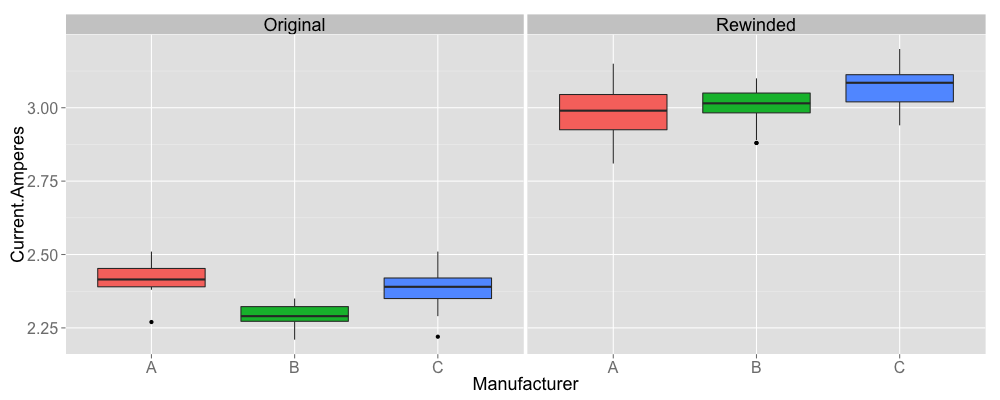
\includegraphics[width=.8\textwidth]{../img/motors_box1.png}
\end{frame}

\begin{frame}[fragile]{Example: Exploratory Data Analysis}

  The exploratory plot suggests a large main effect for the \emph{State} factor,
  and is inconclusive for the effect of the \emph{Manufacturer} factor. It is
  unclear if there are interaction effects or not.\bigskip

  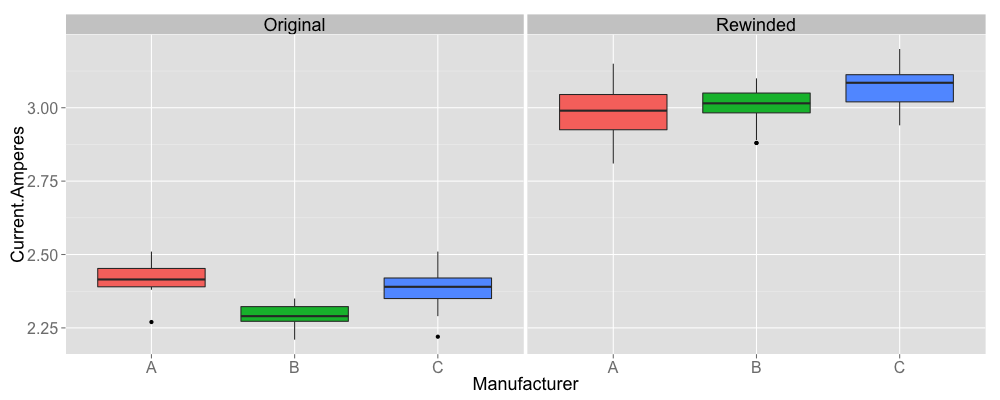
\includegraphics[width=.8\textwidth]{../img/motors_box1.png}
\end{frame}

\begin{frame}{Factorial Design Model}

  In the general case for a completely randomized factorial design we have:

\begin{itemize}
  \item \textit{a} levels for factor \textbf{A};
  \item \textit{b} levels for the factor \textbf{B};
  \item \textit{n} replicates within each combination of levels;
  \item Completely randomized collection of observations;
\end{itemize}\bigskip

  The {\bf additive effects model} for a set of observations collected following this design can be expressed as follows. From this model, we can construct null/alternate hypotheses in a similar fashion as in ANOVA.

  \begin{equation*}
  y_{ijk} = \mu+\tau_i+\beta_j+(\tau\beta)_{ij}+\epsilon_{ijk}\begin{cases}
  i=1,\ldots,a\\
  j=1,\ldots,b\\
  k=1,\ldots,n
\end{cases}\end{equation*}
\end{frame}

\begin{frame}[fragile]{Statistical Model for Two Factors}

The ANOVA gives us the linear model for the mean effect of each
factor (State, Manufacturer), as well as the interaction effect (State x Manufacturer).
\medskip

By analysing these effects, we can define our post-hoc analysis.

{\smaller
\begin{verbatim}
> model <- aov(Current.Amperes~State*Manufacturer,
+              data = data)
> summary(model)
                    Df Sum Sq Mean Sq F value   Pr(>F)
State                1 12.956  12.956 2798.41  < 2e-16 ***
Manufacturer         2  0.118   0.059   12.71 1.04e-05 ***
State:Manufacturer   2  0.114   0.057   12.27 1.49e-05 ***
Residuals          114  0.528   0.005
---

> summary.lm(model)$r.squared
[1] 0.9615174
\end{verbatim}}
\end{frame}

\begin{frame}[fragile]{Examining the Data Assumptions}

As usual, the assumptions can be verified by means of residual analysis, like in the one-way ANOVA (except for a little adjustment needed for the Fligner-Killeen test)

{\smaller
\begin{verbatim}
> shapiro.test(model$residuals)
W = 0.9857, p-value = 0.2392

> fligner.test(Current.Amperes ~ interaction(State, Manufacturer),
+              data = data)
med chi-squared = 10.1721, df = 5, p-value = 0.0705
\end{verbatim}}

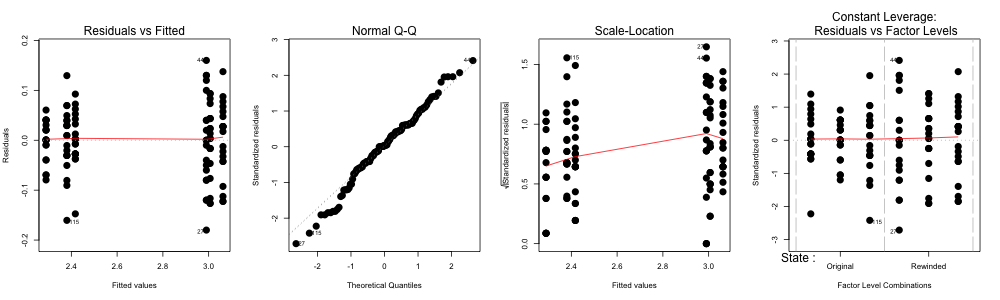
\includegraphics[width=.8\textwidth]{../img/motors_res.png}
\end{frame}

\begin{frame}{Factorial Design -- Post-hoc comparison}

If the ANOVA indicates the existence of significant effects, we can perform pairwise comparisons between levels to investigate specific differences;
\bigskip
When the interaction effect is not significant, the comparisons between factor levels can be done in a straightforward manner, using the estimated level means. For instance, the test statistic for comparing the means of levels 2 and 3 of factor A could be calculated as:

\begin{equation*}
t_0 = \frac{\bar{y}_{2\cdot\cdot} - \bar{y}_{3\cdot\cdot}}{\sqrt{2\frac{MS_E}{n'}}}
\end{equation*}

where $n'$ is the number of specific replicates for the comparison under consideration.
\end{frame}

\begin{frame}[fragile]{Factorial designs -- Post-hoc comparison}

More generally,
\begin{equation*}
t_0 = \frac{\Delta\bar{y}}{\sqrt{2\frac{MS_E}{n'}}}
\end{equation*}

For comparisons of factor levels (main effects), the value of $n'$ is the total number of observations under that level;
\bigskip

For comparisons of level combinations (interaction effects), it is the number of observations within each combination group;

\begin{verbatim}
> replications(Current ~ State*Manufacturer,
+              data = data)
             State       Manufacturer State:Manufacturer
                60                 40                 20
\end{verbatim}

Also, the $\alpha$ value for the comparisons has to be adjusted to prevent inflation of the type-I error rate.
\end{frame}






















%


\section{Recommended Reading}
\begin{frame}{Recommended Reading}
  
  {\bf Block Design}
  \begin{itemize}
    \item D.C. Montgomery, "Design and Analysis of Experiments", Ch4-5
    \item Felipe Campelo, "Design and Analysis of Experiments", Lecture 11
  \end{itemize}

  {\bf Factorial Design}
  \begin{itemize}
    \item Felipe Campelo, "Design and Analysis of Experiments", Chapter 12
    \item Peter Hoff, "Design of Experiment Lecture Notes", Chapter 6
  \end{itemize}
  \vfill

  See links in manaba!
\end{frame}

%%%%%%%%%%%%%%%%%%%%%%%%%%%%%%%%%%%%%%%%%%%%%%%%%%%%
\section{Backmatter}
\begin{frame}{About these Slides}
  These slides were made by Claus Aranha, 2022. You are welcome to copy, re-use and modify this material.
  \bigskip

  These slides are a modification of "Design and Analysis of Experiments (2018)" by Felipe Campelo, used with permission.
  \bigskip

  Individual images in some slides might have been made by other
  authors. Please see the following references for those cases.
\end{frame}

\begin{frame}[allowframebreaks]{Image Credits}
  \printnotes
\end{frame}

\end{CJK}
\end{document}
